\subsection{Тенденции изменения энергий ионизации для различных сэндвичевых соединений}
\subsubsection{Циклопентадиенил}
\textbf{Нарисовать для правильного ответа достаточно лишь выделенное красным}

Потенциалы ионизации объясняются исходя из диаграммы МО сэндвичевых соединений. Для $Cp$ закономерность: потенциал ионизации уменьшается до кобальтоцена, а затем возрастает. 


\begin{figure}[H]
\centering
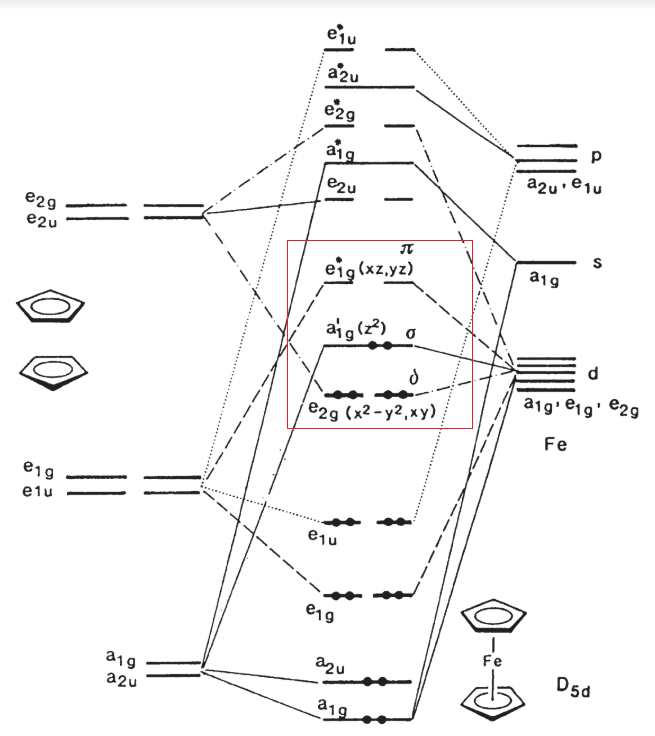
\includegraphics[scale=.600]{images/Cp2Feorb.png}
\end{figure}

Потенциал ионизации кобальтоцена близок к натрию, так как у него имеется один электрон на разрыхляющей орбитали $e_{1g}$, который выгодно отдать и образовать 18-ти электронную конфигурацию. К тому же $e_{1g}$ орбиталь близка по энергии к s орбитали металла (если бы кобальт был s металлом, то электрон уходил бы именно оттуда). 
У манганоцена потенциал ионизации больше (не намного), чем у ферроцена, так как меньше электронов на несвязывающей орбитали.

Хромоцен (16-ти электронная система) – заполнено $e_{2g}$. Потенциал ионизации так же больше, чем у ферроцена и манганоцена. 
У никелоцена 20 электронов, по одному электрону на $e_{1g}$ орбиталях (не выгодно по энергии). Потенциал ионизации никелоцена больше, чем у кобальтоцена, так как у кобальтоцена при отрывании одного электрона образуется выгодная конфигурация с 18 электронами (резкий выигрыш по энергии) в отличие от никелоцена, у которого при отрывании остается один электрон на разрыхляющей орбитали. 
Потенциалы ионизации сэндвичей ранних переходных металлов (до кобальтоцена) в целом несильно отличаются друг от друга. Чем меньше электронов, тем сложнее их оторвать и тем больше потенциал ионизации. 

\subsubsection{Бензол}

Закономерность изменения потенциала ионизации: уменьшается до дибензолмарганца, а затем возрастает. 

\begin{figure}[H]
\centering
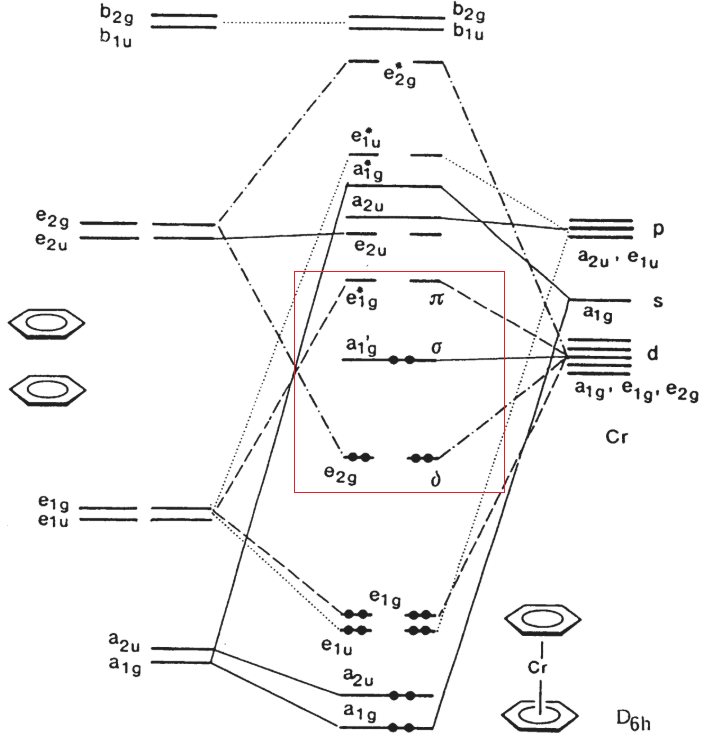
\includegraphics[scale=.600]{images/Benzol2Chromeorb.png}
\caption{}
\label{}
\end{figure}
Чем меньше электронов – тем больше потенциал ионизации. Однако у дибензолмарганца появляется неспаренный электрон на разрыхляющей, что создает невыгодную по энергии ситуацию – электрон легче отдать – энергия ионизации уменьшается. Дальнейшее заполнение e1g орбиталей приводит к увеличению энергии ионизации – отдавать электрон уже не так выгодно, так как это не приводит к образованию устойчивой 18-ти электронной конфигурации. 
Если рассмотреть ферроцен и дибензолхром – у дибензолхрома при ионизации электроны уходят с $a_{1g}$ орбитали, которая находится на уровне d орбиталей хрома, а у ферроцена эта орбиталь на уровне d орбиталей железа. У хрома энергия $d$-орбитали выше, чем у железа, следовательно, электрон проще оторвать от хрома, чем от железа. У дибензолхрома оторвать электрон легче, чем у ферроцена. 
Когда у металла имеется положительный заряд (как в случае с $Cp$), оторвать электрон сложнее - у ферроцена сложнее оторвать электрон. 


